\chapter{Le minimum à maîtriser pour survivre avec Git}\label{chapMinimum} % TODO
% TODO obtenir de l'aide
\index{git@\texttt{git}!help@\texttt{help}}

\section{Enregistrer et lister des modifications} %TODO
% TODO staging, add, rm commit, log
\index{git@\texttt{git}!commit@\texttt{commit}}
\index{git@\texttt{git}!log@\texttt{log}}
\index{historique}
\index{git@\texttt{git}!add@\texttt{add}}
\index{git@\texttt{git}!rm@\texttt{rm}}

\section{Gestion des fichiers non versionnés} % TODO
% TODO .gitignore
\index{ignorer un fichier}
\index{.gitignore@\texttt{.gitignore}}

\section{Gestion des branches} % TODO
% TODO .gitignore
\index{branche}
\index{git@\texttt{git}!branch@\texttt{branch}}
\index{git@\texttt{git}!checkout@\texttt{checkout}}

\section{Travailler avec un dépôt distant} % TODO 
% TODO clone, push, pull, fetch, merge
\index{depot@dépôt!distant}
\index{git@\texttt{git}!clone@\texttt{clone}}
\index{git@\texttt{git}!push@\texttt{push}}
\index{git@\texttt{git}!pull@\texttt{pull}}
\index{git@\texttt{git}!fetch@\texttt{fetch}}
\index{git@\texttt{git}!merge@\texttt{merge}}

\section{Résolution des conflits} %TODO

\index{git@\texttt{git}!merge@\texttt{merge}}
\index{conflit}
% La figure~\ref{fig:conflitGit} illustre l'apparition d'un conflit au
% cours d'un développement en équipe. À un instant donné, le dépôt
% commun aux deux développeurs contient les révisions $A$ et $B$. Le
% premier développeur va commencer un travail sur cette base, et
% produire les révisions $C1$ et $D1$.

% \begin{figure}[h!]
%   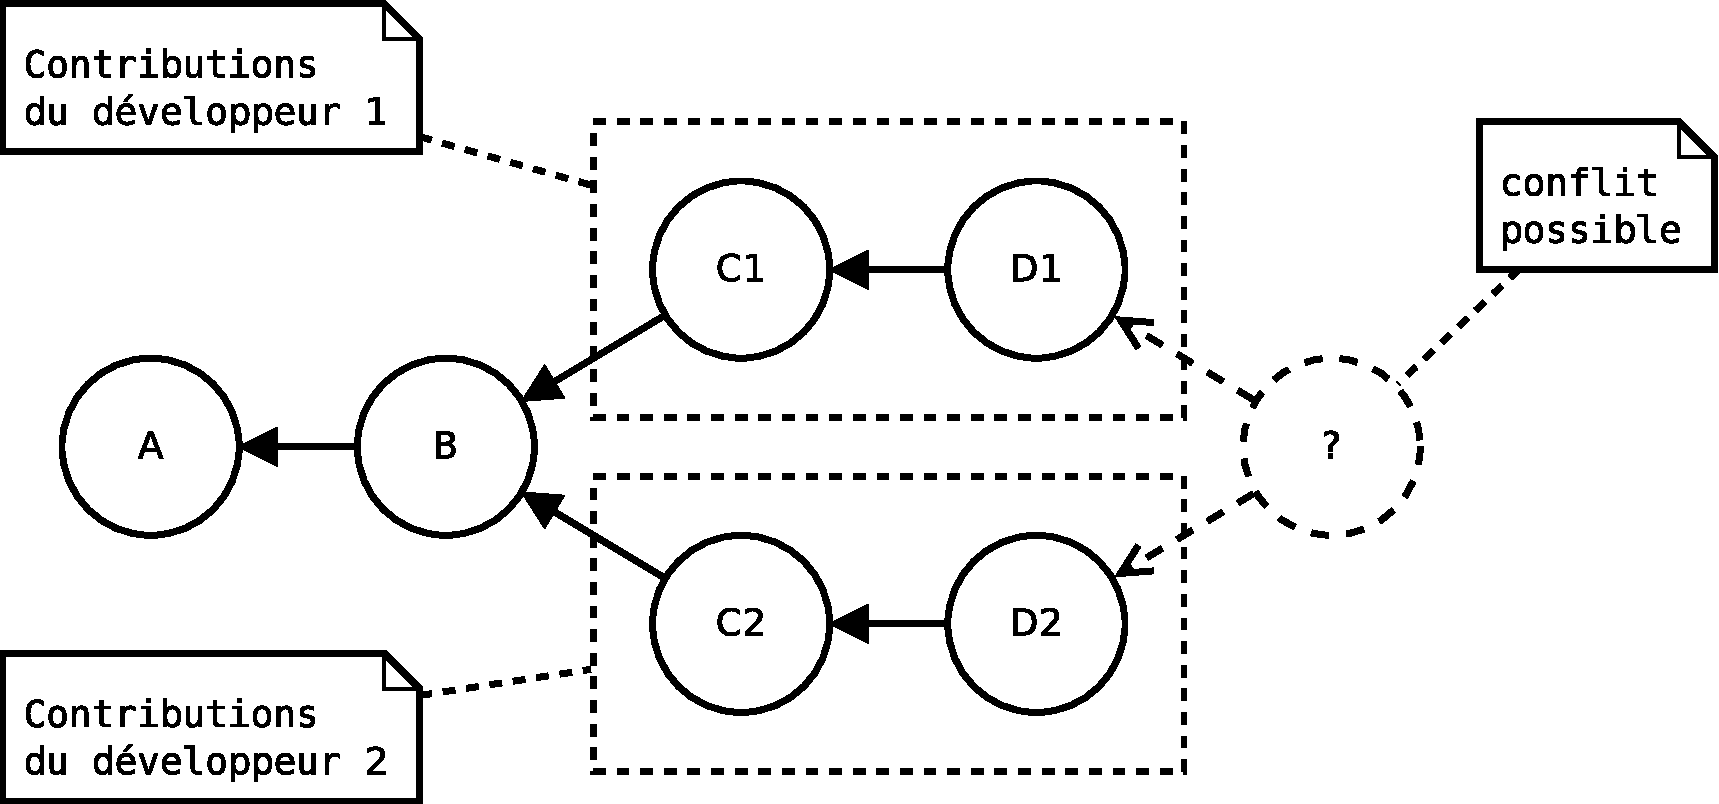
\includegraphics[width=12cm]{figures/conflitGit}
%   \caption{Apparition d'un conflit potentiel entre les contributions
%     de deux développeurs.\label{fig:conflitGit}}
% \end{figure}

\section{Gestion des \textit{tags}} % TODO 
% TODO navigation dans l'historique, reset, revert
% TODO branches, navigation entre branches
% TODO fusion et gestion des conflits
\index{tag@\textit{tag}}
\index{git@\texttt{git}!tag@\texttt{tag}}
\index{git@\texttt{git}!reset@\texttt{reset}}
\index{git@\texttt{git}!revert@\texttt{revert}}
\index{historique}
\index{git@\texttt{git}!branch@\texttt{branch}}
\index{branche}
\index{git@\texttt{git}!checkout@\texttt{checkout}}